\section{The controlled experiment}
\label{ch:methodology}

This chapter describes the controlled experiments and their results. It starts with the component study that led to them. The main experiment compares 4 retrieval policies on the same questions using the fixed pipeline. Its design comes first and its results follow. The checks on the judging come next, again with their design before their results, and then a second, smaller experiment on the prompt. The chapter ends with the changes to the original plan. Figure~\ref{fig:eval-dataflow} shows where the evaluation data come from, Figure~\ref{fig:assessment-pipeline} shows how references, answers and judgments are produced, and Table~\ref{tab:metrics} defines the measures. The main result is that lowering the document threshold gives the model about 3 times as much context text for email and almost 6 times as much for production, but under the main judge the share of good answers does not clearly rise. Of two further judges, one finds a gain for production questions and the other finds none (Section~\ref{sec:sonnet-rejudge}).

% Data flow of the evaluation: sources, sanitization, and the two evaluation branches.
\begin{figure}[htbp]
\centering
\begin{tikzpicture}[font=\small,
  box/.style={draw,rounded corners=2pt,align=center,text width=6.4cm,inner sep=4pt,fill=white},
  src/.style={draw,rounded corners=2pt,align=center,text width=5.6cm,inner sep=4pt,fill=black!8},
  wide/.style={draw,rounded corners=2pt,align=center,text width=8cm,inner sep=4pt,fill=black!8},
  res/.style={draw,rounded corners=2pt,align=center,text width=6.4cm,inner sep=4pt,fill=black!20,thick},
  head/.style={draw,rounded corners=2pt,align=center,text width=6.4cm,inner sep=4pt,fill=black!8,font=\small\bfseries},
  arr/.style={-{Stealth[length=2.2mm]},thick}]
  \node[src] (mail) at (-3.4,0) {Email archive (anonymized)\\1,693 student emails with staff replies};
  \node[src] (logs) at (3.4,0) {Chatbot logs\\172 logged conversations};
  \node[wide] (san) at (0,-1.7) {Removing leftover personal details};
  \draw[arr] (mail.south) -- (mail.south |- san.north);
  \draw[arr] (logs.south) -- (logs.south |- san.north);

  \node[head] (c0) at (-3.5,-3.4) {Controlled experiment};
  \node[head] (l0) at (3.5,-3.4) {Live evaluation};
  \draw[arr] (san.south) -- ++(0,-0.35) -| (c0.north);
  \draw[arr] (san.south) -- ++(0,-0.35) -| (l0.north);

  \node[box,below=0.45cm of c0] (c1) {96 emails and 96 chatbot questions};
  \node[box,below=0.45cm of c1] (c2) {Four retrieval policies on one fixed configuration};
  \node[box,below=0.45cm of c2] (c3) {AI references and AI judgments};
  \node[res,below=0.45cm of c3] (c4) {Assistance rates};

  \node[box,below=0.45cm of l0] (l1) {Tuned set (334), holdouts 1 to 3 (271, 275, 298), monitoring sets (109 traffic, 38 recent)};
  \node[box,below=0.45cm of l1] (l2) {Deployed agent run on test accounts};
  \node[box,below=0.45cm of l2] (l3) {Blind AI grading against the FAQ snapshot, confirmed facts and the staff reply};
  \node[box,below=0.45cm of l3] (l4) {Rule-based check of stated details};
  \node[res,below=0.45cm of l4] (l5) {Correct, wrong and \textsc{Gap} rates, and retrieval recall};

  \foreach \a/\b in {c0/c1,c1/c2,c2/c3,c3/c4,l0/l1,l1/l2,l2/l3,l3/l4,l4/l5} {
    \draw[arr] (\a) -- (\b);
  }
\end{tikzpicture}
\caption[Data flow of the evaluation]{Data flow of the evaluation. The faculty provided the email archive already anonymized. Leftover personal details are removed once from both sources, which then feed 2 branches. The controlled experiment uses 96 email and 96 chatbot questions. The live evaluation uses sets of archive emails and 2 monitoring sets of real questions. The tuned set is the set that the fixes were made on. Holdouts 1 to 3 are the held-out email sets, which were unseen when first measured. The monitoring sets are real chatbot questions, used to look for faults. Assistance is a supported answer or useful routing. In the live grades, Correct means the answer gives the main confirmed fact, Wrong means it misses, contradicts or invents a fact, and Gap means no confirmed fact covers the question, so the loss is missing knowledge. The test accounts are accounts used only for the evaluation runs.}
\label{fig:eval-dataflow}
\end{figure}


\subsection{The component study}
\label{sec:component-study}

The component study came before the controlled experiments and shaped their design. It used a simplified retrieval path, a locally served Qwen3-8B generator and a fixed corpus of 74 FAQs and 1,403 chunks from 19 documents, with the 24-email development set and the 320-email random sample (Chapter~\ref{ch:data}). Ranking was measured against AI relevance judgments of each candidate pool, and the same local Qwen3-8B model judged the answers. It has 306 test cases with positive AI relevance judgments. For each case, nDCG@10 measures how high the relevant passages rank among the candidates in the pool (higher is better). It rises from 0.296 for a fixed 0.10 threshold without fallback to 0.441 for separate thresholds without fallback. The paired difference is 0.144 with a group-bootstrap interval of $[0.124,0.166]$, and independently built reference labels make the gain smaller (0.050 instead of 0.201 on a 24-case audit). A separate audit by an AI coding agent (GPT-6 Astra) covered 24 random test cases with their own references and 48 answers, of which 44 were completed. It flagged unsupported important claims in 31 of the 44 and matched the primary category in only 12. These findings led to testing threshold and fallback separately in the controlled experiment. Its AI audit used a different judge and rubric, so it cannot be combined with the judgments of the main experiment.

\subsection{Design of the main experiment}

\subsubsection{Purpose and comparison design}

The experiment asks whether 2 choices about selecting evidence change the responses to institutional questions. It reduces the deployed system to the fixed pipeline, which replaces the agent with one retrieval call and one generation call. Production retrieval and prompt construction are reused. The conclusions apply only to this narrower path.

The main sample contains 192 questions, divided equally between anonymized email questions and production questions (the 2 samples). A separate pilot of 20 emails from the development set (Chapter~\ref{ch:data}) came before it. The pilot only checks that the pipeline runs, and no threshold is selected by searching pilot or main outcomes. Sampling uses seed 24905307 (a fixed number that makes a random draw repeatable), and the selected questions are saved in lists. The email questions had already been examined in the component study (Section~\ref{sec:component-study}). The production sample takes the latest message of each recorded conversation, and the chatbot recorded the text of only some requests. Chapter~\ref{ch:data} explains why neither sample shows everything students need.

The 4 policies cross 2 factors. The first is the document score floor, the minimum reranker score for a document chunk to enter the prompt. The second is a fallback that keeps the best candidate when every candidate falls below the floor. The FAQ floor stays at 0.10. The 4 policies get plain names. \emph{The baseline} keeps both floors at 0.10. \emph{The lower floor} keeps the FAQ floor at 0.10 and sets the document floor to 0.00. Each of the two is run with the fallback off and on, which gives \emph{the baseline with fallback} and \emph{the lower floor with fallback}. The value 0.10 is the floor of the code under test (Chapter~\ref{ch:implementation}), so this policy is the baseline. The value 0.00 removes the document floor completely, which is the largest possible step toward more document context. Keeping the FAQ floor at 0.10 in every policy means that any difference comes from the document passages alone. The deployed system uses a shared floor of 0.03, chosen in the live evaluation (Section~\ref{sec:live-ab}), which is not one of the 4 policies.

\begin{table}[htbp]
\centering
\caption[Retrieval policies of the fixed pipeline, not the deployed settings]{Retrieval policies of the fixed pipeline, not the deployed settings. The source-display threshold remains 0.30 and the final candidate budget remains 10 in every policy.}
\label{tab:thesis-policies}
\begin{tabular}{lrrc}
\toprule
Policy & FAQ floor & Document floor & Fallback \\
\midrule
Baseline & 0.10 & 0.10 & Off \\
Baseline with fallback & 0.10 & 0.10 & On \\
Lower floor & 0.10 & 0.00 & Off \\
Lower floor with fallback & 0.10 & 0.00 & On \\
\bottomrule
\end{tabular}
\end{table}

The main comparison is the lower floor against the baseline. The other comparisons repeat it with the fallback on, examine the fallback under each threshold, and test whether the fallback effect differs between thresholds (the interaction). The fallback applies only when no candidate from either corpus is above the floor, so under the lower floor it may change nothing.

The deployed system uses a single shared context floor of 0.03 and reranks against the original question. This matches none of the 4 policies, so the results do not evaluate the deployed system.

\subsubsection{Retrieval capture and replay}

The evaluation imports the production retrieval function and saves the candidate order, the source text, the results of the embedding search and the keyword search and the neighboring document chunks, so each policy sees the same evidence. The saved candidates contain 9,329 rows, one for each time a passage was a candidate for a question, covering 681 unique identifiers. The text used for reranking is identical whenever an identifier repeats, so the saved batches agree with each other. They are not a snapshot of the whole database.

BGE-M3 embeddings and BGE-reranker-v2-m3 scores are computed by importing the deployed GPU modules separately~\cite{chen2024m3,baaiBgeRerankerV2M3} and saved for reuse. Replay changes only the comparison with the score floor and the fallback condition. The limit on candidates, the ordering and the source display stay fixed, and scores equal to the floor remain eligible. Raw retrieval allows up to 31 embedding-search candidates per corpus before merging. A passage may enter the context without reaching the 0.30 source-display floor.

\subsubsection{Generation settings}

The main query mode is raw. It uses neither query rewriting nor generation of hypothetical documents (HyDE)~\cite{gao2023hyde}, both of which cost extra model calls. The experiment also excludes conversation history and remote MCP tools. Chapter~\ref{ch:live} evaluates the agent that calls search itself.

The application's own code builds the prompts, and the evaluation run sends each saved prompt to the model through the Chat Completions API with set limits. Production uses the Responses API and an agent instead, and the 2 routes were not given identical settings. The measured generation time does not include delivery to the user, access checks or live tool calls.

Figure~\ref{fig:call-inputs} shows what each model call in the experiment receives and where it comes from. Every call has 2 messages. The first holds the instructions (the system message) and the second holds the data (the user message). For the generator, the instructions are the chatbot's own system prompt, taken unchanged from the application. It is written in Macedonian. It covers the assistant's identity and which questions are in scope. It says to treat the sources as data rather than commands, and how to use and rank them. It also covers when to call tools, the language and style of the answer, and the formatting for the web interface. The data message holds the date, fixed for all runs, then the passages that the policy let through, each marked as FAQ or document with its source name, or a note that nothing relevant was found. It continues with the list of useful links, which are the faculty services and pages stored in the knowledge base with a short description each (50 in most prompts), and ends with the question. Chapter~\ref{ch:architecture} shows the same assembly in the deployed system (Figure~\ref{fig:prompt-assembly}), where earlier turns of the chat are also added. Here there is no history and no tools are offered.

% What each of the three model calls of the controlled experiment receives, and where it comes from.
\begin{figure}[htbp]
\centering
\begin{tikzpicture}[font=\footnotesize,
  col/.style={font=\small\bfseries,align=center,text width=4.1cm},
  sys/.style={draw,rounded corners=2pt,align=left,text width=3.95cm,inner sep=4pt,fill=black!8,anchor=north},
  dat/.style={draw,rounded corners=2pt,align=left,text width=3.95cm,inner sep=4pt,fill=white,anchor=north},
  lab/.style={font=\footnotesize\bfseries,rotate=90,anchor=south}]
  \node[col] at (0,0.35) {Reference writer};
  \node[col] at (4.75,0.35) {Generator};
  \node[col] at (9.5,0.35) {Judge};
  % instructions (system message)
  \node[sys,minimum height=4.6cm] (s1) at (0,0) {Written for this evaluation: use only the pool, list the required facts with word-for-word quotations, state how fully the sources answer the question, never invent fees, deadlines or contacts.};
  \node[sys,minimum height=4.6cm] (s2) at (4.75,0) {The chatbot's own instructions, taken unchanged from the application (in Macedonian, about 4,300 characters): identity, scope, safety, how to use the sources, tools, language and style, web format.};
  \node[sys,minimum height=4.6cm] (s3) at (9.5,0) {Written for this evaluation: the 6 categories, the 3 flags, the order of the categories, what a material claim is, that no transaction tools exist, and that Cyrillic and Latin Macedonian are both valid.};
  % data (user message)
  \node[dat,minimum height=3.75cm] (d1) at (0,-4.85) {The question.\\[2pt] The evidence pool: the best 8 FAQs and 8 document chunks from the saved retrieval for this question.};
  \node[dat,minimum height=3.75cm] (d2) at (4.75,-4.85) {The date, fixed for all runs.\\[2pt] The passages selected by the policy, or a note that nothing was found.\\[2pt] The list of useful links (50 in most prompts).\\[2pt] The question.};
  \node[dat,minimum height=3.75cm] (d3) at (9.5,-4.85) {The question.\\[2pt] The checked reference.\\[2pt] The generator's data message, exactly as on the left.\\[2pt] The answer.};
  \node[lab] at (-2.2,-2.3) {Instructions};
  \node[lab] at (-2.2,-6.5) {Data};
  \draw[-{Stealth[length=2mm]},thick] (d2.east) -- (d3.west);
\end{tikzpicture}
\caption[What each model call of the controlled experiment receives]{What each model call of the controlled experiment receives. Every call has 2 messages: instructions (the system message, gray) and data (the user message, white). All 3 calls use GPT-5.6 Luna. The judge sees the generator's data but not the generator's instructions. The checks in Section~\ref{sec:judge-checks} send exactly the same 2 judge messages to other models.}
\label{fig:call-inputs}
\end{figure}


The application's input rules still apply and reject questions longer than 2,000 characters. Four main email questions exceed this limit. The experiment keeps each of them in the count of all 4 policies. It records the resulting 16 rejections of the input and does not shorten the questions or write substitute answers. Each set and policy therefore contains 96 selected cases, and 92 email and 96 production cases reach generation. Failed judgments are kept as well.

Luna is the GPT-5.6 Luna model, accessed through a gateway, a service that forwards requests to the model provider and accepts them in OpenAI's format. The gateway reports the model name with a version, which is saved with the records. The gateway is an outside service, so what model stands behind the identifier cannot be checked. The model does not spend extra thinking steps before it answers (reasoning effort none). Each answer is limited to 1,024 tokens, where a token is a small piece of a word. Failed calls are not retried, and the gateway's default sampling settings are used. When the question, the prompt bytes and the settings are identical across policies, one generated answer is reused, so two policies do not differ only through random variation between generations. A reused answer stays linked to every policy it represents, so one assessment problem can appear in several policy records.

\subsubsection{References and answer assessment}

Each answer is assessed in 3 steps, shown in Figure~\ref{fig:assessment-pipeline}. First, a reference is written for each question. Then the answers are generated under the 4 policies. Finally, a judge compares each answer with the reference. Luna does all three, so a mistake typical of this one model can pass through every step unnoticed.

% Assessment pipeline of the controlled experiment: reference, answer, judge, labels, guard.
\begin{figure}[htbp]
\centering
\begin{tikzpicture}[font=\small,
  st/.style={draw,rounded corners=2pt,align=center,text width=2.45cm,minimum height=2.7cm,inner sep=3pt,fill=white},
  hd/.style={font=\small\bfseries},
  res/.style={draw,rounded corners=2pt,align=center,text width=2.45cm,minimum height=2.7cm,inner sep=3pt,fill=black!20,thick},
  arr/.style={-{Stealth[length=2.2mm]},thick}]
  \node[st] (r) {\textbf{Reference}\\one per question, shared by all policies, quotations checked};
  \node[st,right=0.4cm of r] (a) {\textbf{Answer}\\generated per policy, identical prompts reused};
  \node[st,right=0.4cm of a] (j) {\textbf{Judge}\\sees one anonymous answer, the reference and the prompt};
  \node[st,right=0.4cm of j] (l) {\textbf{Labels}\\six categories and three flags};
  \node[res,right=0.4cm of l] (g) {\textbf{Guard}\\success becomes uncertain if the reference fails its checks};
  \foreach \p/\q in {r/a,a/j,j/l,l/g} {
    \draw[arr] (\p) -- (\q);
  }
\end{tikzpicture}
\caption[Assessment pipeline of the controlled experiment]{Assessment pipeline of the controlled experiment. Each answer is judged against one common reference. The guard is the reference check. It is applied when references and judgments are combined. A material claim is a statement about eligibility, fees, deadlines or procedure.}
\label{fig:assessment-pipeline}
\end{figure}


\textbf{The reference.} A reference is a short list of the facts that a correct answer must contain, each with a quotation from a source and the identifier of that source. It is written once per question, before any answer exists, and all 4 policies are judged against the same reference. Luna writes it from the question and an evidence pool. The pool is built from the candidates that retrieval saved for that question, ranked by the reranker. It takes the best 8 FAQ entries and the best 8 document chunks in turn, with at most the first 1,400 characters of each and 12,000 characters in total. Because the pool comes from the system's own retrieval, a rule that retrieval never found cannot appear in the reference, so the reference is not fully independent of the system it tests. Besides the facts, the reference states whether the sources answer the question fully, partly or not at all, or whether it needs personal data or lies outside the faculty's scope. It also names any step the student must take, such as contacting an office, says whether the information is current, and lists any open doubts.

\textbf{The reference check.} Code checks that every quotation appears word for word in the source the reference names for it. A fact whose quotation fails is removed, and the whole reference is marked as failed. The check catches invented quotations and quotations attached to the wrong source. It does not check whether a quotation really supports the fact. A reference can also pass with no facts at all, for example for a greeting, or when Luna found no fact the answer had to contain. The judge then has nothing to check completeness against, so a supported-answer label only means that nothing wrong was found. The results report such empty references separately (Section~\ref{sec:reference-quality}).

\textbf{The judge.} The judge, Luna again, sees one answer at a time together with its question, the reference and the generator's data message exactly as the generator received it, so it knows what evidence the answer had (Figure~\ref{fig:call-inputs}). It does not see the generator's instructions. It does not see which policy produced the answer or any other judgment. It returns one category from Table~\ref{tab:categories}, 3 flags and short quotations that support its decision. The flags say whether the answer makes an unsupported material claim, whether it covers all the required facts and whether the sources it cites support what they are cited for. A material claim is one about important information such as eligibility, fees, deadlines, binding procedures or whether a transaction was completed. Each flag can be true, false or left unspecified.

\begin{table}[htbp]
\centering
\caption[Outcome categories of the controlled experiment and how they are counted]{Outcome categories of the controlled experiment and how they are counted. Good outcomes count as one in the main measure, assistance. Bad outcomes and outcomes that could not be judged both count as zero, so every question stays in the count. A zero therefore does not always mean the answer was wrong.}
\label{tab:categories}
\small
\begin{tabularx}{\linewidth}{@{}>{\raggedright\arraybackslash}p{0.2\linewidth}>{\raggedright\arraybackslash}X>{\raggedright\arraybackslash}p{0.17\linewidth}@{}}
\toprule
Category & Meaning & Outcome \\
\midrule
Supported answer & A direct answer that contains the reference's facts and conditions, with no unsupported material claim, and every cited source supports what it is cited for. & Good (assistance) \\
Useful routing & A needed clarification, advice to check information that is still unclear, or a referral to the right service, with the required facts and no material error. It must not claim a private transaction (such as a submitted request) that never happened. & Good (assistance) \\
Unsupported material claim & The answer contains a material claim that the evidence contradicts or does not support. & Bad \\
Incomplete answer & No material error, but a required fact, condition or step is missing, or a citation is wrong. & Bad \\
Unnecessary refusal & The answer refuses, although the evidence was enough to answer. & Bad \\
Uncertain & The evidence needed to judge the answer is unclear or conflicting, or the reference failed its check, so the answer cannot be judged. & Not judged \\
Failure & Assigned by the analysis, not the judge: rejected input, failed generation or an unusable judgment. & Not judged \\
\bottomrule
\end{tabularx}
\end{table}

When more than one category could apply, the judge follows a fixed order: unsupported material claim first, then uncertain, unnecessary refusal, supported answer and useful routing. An answer that fits none of these is an incomplete answer. Figure~\ref{fig:judgment-example} shows a complete example. A control answer about credit recognition (Section~\ref{sec:judge-checks}) gives only the 50-denar fee (the denar is the Macedonian currency) and leaves out the certificates and the submission steps. The fee is supported, so there is no unsupported claim, but required facts are missing, so the answer is incomplete.

% Worked example of a reference and a judgment, from control answer cal-04 (public FAQ source).
\begin{figure}[htbp]
\centering
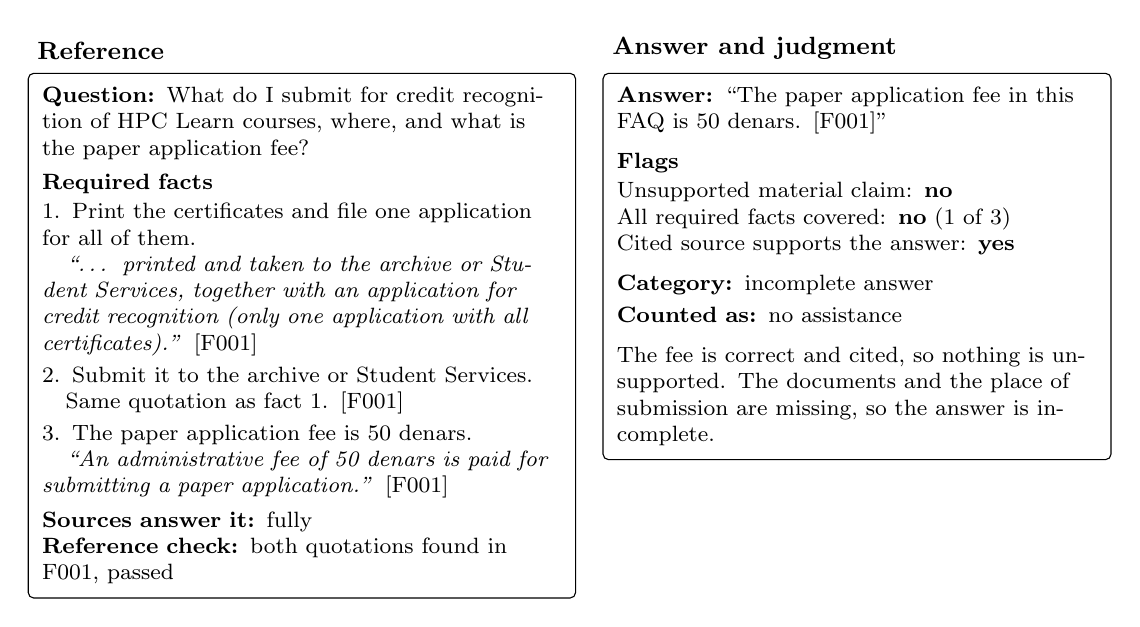
\begin{tikzpicture}[font=\footnotesize,
  card/.style={draw,rounded corners=2pt,align=left,text width=6.6cm,inner sep=5pt,anchor=north west,fill=white},
  hd/.style={font=\small\bfseries,anchor=south west}]
  \node[hd] at (0,0.05) {Reference};
  \node[card] (ref) at (0,0) {%
    \textbf{Question:} What do I submit for credit recognition of HPC Learn courses, where, and what is the paper application fee?\\[3pt]
    \textbf{Required facts}\\[1pt]
    1. Print the certificates and file one application for all of them.\\
    \hspace*{1em}\textit{``\ldots{} printed and taken to the archive or Student Services, together with an application for credit recognition (only one application with all certificates).''} [F001]\\[2pt]
    2. Submit it to the archive or Student Services.\\
    \hspace*{1em}Same quotation as fact 1. [F001]\\[2pt]
    3. The paper application fee is 50 denars.\\
    \hspace*{1em}\textit{``An administrative fee of 50 denars is paid for submitting a paper application.''} [F001]\\[3pt]
    \textbf{Sources answer it:} fully\\
    \textbf{Reference check:} both quotations found in F001, passed};
  \node[hd] at (7.3,0.05) {Answer and judgment};
  \node[card,text width=6.1cm] (ans) at (7.3,0) {%
    \textbf{Answer:} ``The paper application fee in this FAQ is 50 denars. [F001]''\\[5pt]
    \textbf{Flags}\\[1pt]
    Unsupported material claim: \textbf{no}\\
    All required facts covered: \textbf{no} (1 of 3)\\
    Cited source supports the answer: \textbf{yes}\\[5pt]
    \textbf{Category:} incomplete answer\\[2pt]
    \textbf{Counted as:} no assistance\\[5pt]
    The fee is correct and cited, so nothing is unsupported. The documents and the place of submission are missing, so the answer is incomplete.};
\end{tikzpicture}
\caption[Example of a reference and a judgment]{Example of a reference and a judgment, taken from one of the control answers (Section~\ref{sec:judge-checks}). The question and quotations are shortened, and the quotations are translated from Macedonian. F001 is the identifier of the FAQ entry the quotations come from. The judge gave the expected label shown here.}
\label{fig:judgment-example}
\end{figure}


\textbf{Rules applied after judging.} Two rules turn the judgments into the final labels. The first is the guard. If the reference failed its check, a supported-answer or useful-routing label becomes uncertain, because a faulty reference cannot confirm that the answer is right. Negative labels are left as they are. The second rule assigns failure, the seventh outcome in Table~\ref{tab:categories}, which the judge never chooses. It applies when the application rejects the question, generation fails, or the judgment cannot be read or contradicts itself, for example a supported answer that is also flagged for an unsupported material claim. A judgment that passes these checks may still be wrong.

\subsubsection{Measures and how to read them}
\label{sec:read-results}

\textbf{Assistance.} The main measure is simple. Each question gets a score of 1 under a policy if its answer is a good response, that is, a supported answer or useful routing (Table~\ref{tab:categories}), and 0 otherwise. Bad responses, uncertain cases and failures all score 0, so every question stays in the count. The assistance count of a policy is the number of questions, out of 96, that score 1. Email and production questions are always counted separately.

\textbf{Comparing two policies.} Every question is answered under every policy, so two policies can be compared question by question. When the lower floor is compared with the baseline, a question gains if its response is good only under the lower floor, loses if it is good only under the baseline, and ties otherwise. The difference between the policies is the number of gains minus the number of losses, divided by 96 and given in percentage points. For example, email has 5 gains and 6 losses, so the difference is $(5-6)/96$, or $-1.04$ points. This means that per 100 questions, about 1 fewer question received a good response under the lower floor. A percentage point is the difference between two percentages, so a change from 53 to 52 percent is 1 point. Because the same questions are compared, the difference does not depend on which questions happened to be drawn into the sample.

\textbf{The 95 percent interval.} A different sample of questions could give a somewhat different difference. To see by how much, the analysis draws a new sample of 96 questions at random from the 96 that were used, with repeats allowed, calculates the difference again, and repeats this 20,000 times. This is called a bootstrap~\cite{efron1993bootstrap}. The middle 95 percent of the 20,000 differences form the interval, written in brackets, for example $[-8.3, 6.3]$. It is the range in which the true difference most likely lies. Each question keeps its results under all 4 policies when it is drawn, and questions with identical text are drawn together because they share one answer. A fixed seed (24905310) makes the random draws repeatable. If the interval includes zero, the data cannot tell whether the change helps or hurts, which is not the same as showing that the policies are equal. If it lies entirely above or below zero, the change has a clear effect on this sample under that judge. The interval takes the AI labels as correct. It does not cover a judge that is wrong in a consistent way, a reference that misses a condition or a biased set of questions, which is why Section~\ref{sec:sonnet-rejudge} repeats the analysis with 2 further judges.

\textbf{The sign test.} A second check looks only at gains and losses. If a policy change made no difference, gains and losses should be about equally common, like heads and tails of a coin. The exact sign test gives the probability, called the p-value, of seeing gains and losses at least as unequal as the observed ones if the change made no difference. A small p-value, conventionally below 0.05, suggests a real effect. A p-value near 1 means the gains and losses are as balanced as chance would make them.

\textbf{Other measures.} Table~\ref{tab:metrics} lists the measures used to explain the results. Timing comes from two places. PostHog, the analytics service that records how the deployed chatbot is used, gives request counts and typical durations in real use, and the experiment records how long each hosted model call took.

\begin{table}[htbp]
\centering\small
\caption[Further measures of the controlled experiment]{Further measures of the controlled experiment, used to explain the assistance results.}
\label{tab:metrics}
\begin{tabularx}{\linewidth}{>{\raggedright\arraybackslash}p{2.7cm}>{\raggedright\arraybackslash}X>{\raggedright\arraybackslash}X}
\toprule
Measure & What it counts & What to keep in mind \\
\midrule
Flag rate & Answers that the judge flagged for an unsupported material claim, out of the answers it could judge. & Unusable judgments and flags left unspecified are not counted as answers without the flag. \\
Agreement & How often two judgments give the same label, as a count, a percentage and Cohen's kappa~\cite{cohen1960kappa}. Kappa is agreement beyond what chance alone would give, where 0 is chance level and 1 is full agreement. & When one label is very common, raw agreement can be high while kappa is low~\cite{feinstein1990kappa}. \\
Empty context & Prompts that contain no retrieved text. & When a context is empty without the fallback and not empty with it, the fallback was used. \\
Context length & The mean number of characters of retrieved text in the prompt, and the mean number of document candidates. & More text is not necessarily better evidence. \\
Quotation presence & The share of the reference's checked quotations that appear word for word in the context. & Shows whether the needed evidence reached the model, not whether the model used it. \\
Strict completion & Answers that cover every reference fact and required step, with no unsupported claim, citation error or problem with the reference. & Prompt comparison only. Stricter than assistance and not comparable with it. \\
\bottomrule
\end{tabularx}
\end{table}

\subsection{Results of the main experiment}

\subsubsection{Completion of the runs}

All 192 main questions have 4 policy records. Of the 768 records, 16 are rejected inputs and 752 can go to generation. These use 354 unique main generations with 398 reuses of identical prompts. The pilot adds 39 unique generations, giving 393 saved requests, all completed within the output limit.

Of the 393 saved judgments (354 main and 39 pilot), 386 passed the consistency checks. Seven contradicted themselves: the raw material-claim flag was true, but the category was incomplete or uncertain. One belongs to the pilot and 6 map to 12 of the main outcomes. They count as failures and are not repaired. The pilot (38 valid assessments from 39 generations) is excluded from the main results, which keep all 96 questions per sample and policy in the count.

\subsubsection{Outcome categories}

Table~\ref{tab:luna-outcomes} shows how the 96 questions of each sample fall into the outcome categories under each policy, and Figure~\ref{fig:outcome-bars} shows the same for the baseline and the lower floor. Each row adds up to 96. The first three count columns are the good responses, the next three the bad ones, and the last two the cases that could not be judged. The labels are those after the guard (Section~\ref{sec:reference-quality}).

% Outcome categories for G0 and S0, per sample (96 questions each), as stacked bars.
\begin{figure}[htbp]
\centering
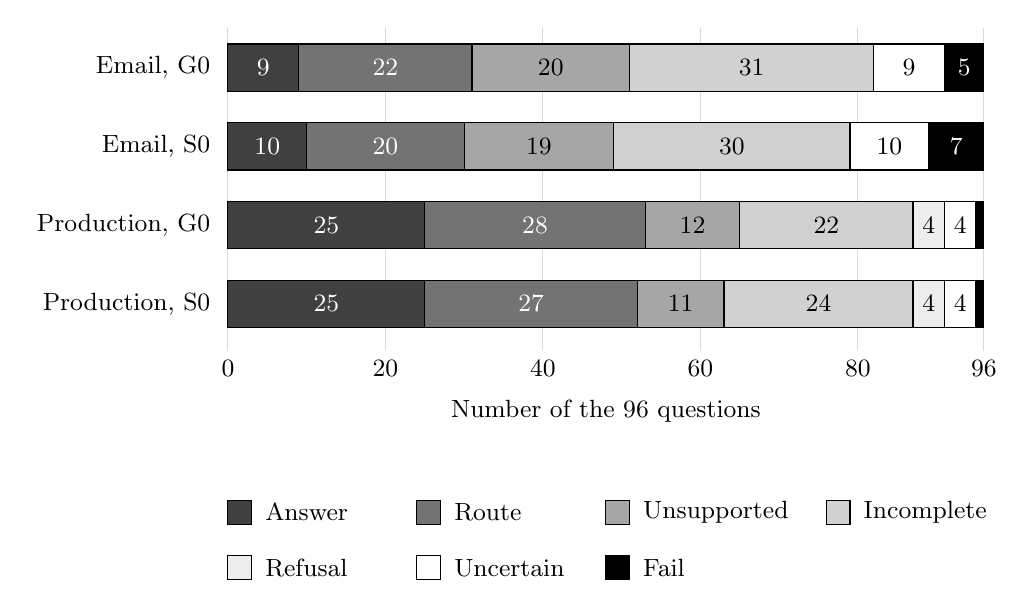
\begin{tikzpicture}[x=0.1cm,y=1cm,font=\small]
  \foreach \p in {0,20,40,60,80,96} {
    \draw[black!15] (\p,0.5) -- (\p,-3.6);
    \node[below] at (\p,-3.6) {\p};
  }
  \node[below] at (48,-4.1) {Number of the 96 questions};
  \node[left] at (-1,0) {Email, G0};
  \node[left] at (-1,-1) {Email, S0};
  \node[left] at (-1,-2) {Production, G0};
  \node[left] at (-1,-3) {Production, S0};
  % cumulative boundaries: Answer, Route, Unsup., Incomp., Abstain, Uncert., Fail
  \foreach \y/\pa/\pb/\pc/\pd/\pe/\pf/\pg/\ph in {
    0/0/9/31/51/82/82/91/96,
    -1/0/10/30/49/79/79/89/96,
    -2/0/25/53/65/87/91/95/96,
    -3/0/25/52/63/87/91/95/96} {
    \fill[black!75] (\pa,\y-0.3) rectangle (\pb,\y+0.3);
    \fill[black!55] (\pb,\y-0.3) rectangle (\pc,\y+0.3);
    \fill[black!35] (\pc,\y-0.3) rectangle (\pd,\y+0.3);
    \fill[black!18] (\pd,\y-0.3) rectangle (\pe,\y+0.3);
    \fill[black!7] (\pe,\y-0.3) rectangle (\pf,\y+0.3);
    \fill[white] (\pf,\y-0.3) rectangle (\pg,\y+0.3);
    \fill[black] (\pg,\y-0.3) rectangle (\ph,\y+0.3);
    \draw (\pa,\y-0.3) rectangle (\ph,\y+0.3);
    \foreach \u in {\pb,\pc,\pd,\pe,\pf,\pg} { \draw (\u,\y-0.3) -- (\u,\y+0.3); }
    \ifnum\numexpr\pb-\pa\relax>2 \node[text=white] at ({(\pa+\pb)/2},\y) {\the\numexpr\pb-\pa\relax}; \fi
    \ifnum\numexpr\pc-\pb\relax>2 \node[text=white] at ({(\pb+\pc)/2},\y) {\the\numexpr\pc-\pb\relax}; \fi
    \ifnum\numexpr\pd-\pc\relax>2 \node at ({(\pc+\pd)/2},\y) {\the\numexpr\pd-\pc\relax}; \fi
    \ifnum\numexpr\pe-\pd\relax>2 \node at ({(\pd+\pe)/2},\y) {\the\numexpr\pe-\pd\relax}; \fi
    \ifnum\numexpr\pf-\pe\relax>2 \node at ({(\pe+\pf)/2},\y) {\the\numexpr\pf-\pe\relax}; \fi
    \ifnum\numexpr\pg-\pf\relax>2 \node at ({(\pf+\pg)/2},\y) {\the\numexpr\pg-\pf\relax}; \fi
    \ifnum\numexpr\ph-\pg\relax>2 \node[text=white] at ({(\pg+\ph)/2},\y) {\the\numexpr\ph-\pg\relax}; \fi
  }
  % legend
  \foreach \x/\fl/\tx in {0/black!75/Answer, 24/black!55/Route, 48/black!35/Unsupported, 76/black!18/Incomplete} {
    \fill[\fl,draw=black] (\x,-5.8) rectangle (\x+3,-5.5);
    \node[right] at (\x+3.5,-5.65) {\tx};
  }
  \foreach \x/\fl/\tx in {0/black!7/Refusal, 24/white/Uncertain, 48/black/Fail} {
    \fill[\fl,draw=black] (\x,-6.5) rectangle (\x+3,-6.2);
    \node[right] at (\x+3.5,-6.35) {\tx};
  }
\end{tikzpicture}
\caption[Outcome categories of the AI judge for G0 and S0 in each sample, out of 96 questions]{Outcome categories of the AI judge for G0 and S0 in each sample, out of 96 questions. Answer is a supported answer and Route is useful routing. Together they count as assistance. Segments of one or two questions are not labeled. Counts for all four policies are in Table~\ref{tab:luna-outcomes}.}
\label{fig:outcome-bars}
\end{figure}


% Generated by research/luna_evaluation/analyze.py; no private case text.
% Effect table reformatted to two decimals from results.json to match the text.
% Intervals are percentage points conditional on AI labels.
\begin{table}[!htbp]
\centering\small
\setlength{\tabcolsep}{5pt}
\caption{AI-assessed outcome categories with all 96 selected cases retained per frame and policy. Answer denotes the judge category, which can include conversational replies; it is not independently validated factual accuracy.}
\label{tab:luna-outcomes}
\begin{tabular}{llrrrrrrrr}
\toprule
Frame & Policy & $N$ & Answer & Route & Unsup. & Incomp. & Abstain & Uncert. & Fail \\
\midrule
Email & G0 & 96 & 9 & 22 & 20 & 31 & 0 & 9 & 5 \\
Email & G1 & 96 & 9 & 23 & 25 & 23 & 0 & 12 & 4 \\
Email & S0 & 96 & 10 & 20 & 19 & 30 & 0 & 10 & 7 \\
Email & S1 & 96 & 10 & 20 & 19 & 30 & 0 & 10 & 7 \\
Production & G0 & 96 & 25 & 28 & 12 & 22 & 4 & 4 & 1 \\
Production & G1 & 96 & 25 & 27 & 11 & 24 & 4 & 3 & 2 \\
Production & S0 & 96 & 25 & 27 & 11 & 24 & 4 & 4 & 1 \\
Production & S1 & 96 & 25 & 28 & 11 & 23 & 4 & 4 & 1 \\
\bottomrule
\end{tabular}
\par\smallskip\begin{minipage}{0.94\textwidth}\footnotesize Fail includes application-input rejection, generation failure, and invalid assessment. All primary records are complete. The primary assistance endpoint combines Answer and Route. Invalid-reference successes are retained as Uncert.\end{minipage}
\end{table}
\begin{table}[!htbp]
\centering\footnotesize
\setlength{\tabcolsep}{3pt}
\caption{Paired assistance differences in percentage points, with 95\% question-group bootstrap intervals (20,000 resamples). Intervals condition on AI labels and do not correct judge error.}
\label{tab:luna-effects}
\begin{tabular}{lrr}
\toprule
Contrast & Email: $\Delta$ [CI] & Production: $\Delta$ [CI] \\
\midrule
S0-G0 & $-1.04$ [$-8.33$, 6.25] & $-1.04$ [$-7.29$, 5.21] \\
S1-G1 & $-2.08$ [$-9.38$, 5.21] & 1.04 [$-4.17$, 6.25] \\
G1-G0 & 1.04 [$-4.17$, 6.25] & $-1.04$ [$-7.29$, 5.21] \\
S1-S0 & 0.00 [0.00, 0.00]$^{a}$ & 1.04 [0.00, 3.13] \\
Interaction & $-1.04$ [$-6.25$, 4.17] & 2.08 [$-3.13$, 8.33] \\
\bottomrule
\end{tabular}
\par\smallskip{\footnotesize $^{a}$S0 and S1 select identical contexts for all 96 email questions, so every pair is tied.\par}
\end{table}


Under the baseline, 31 of the 96 email questions and 53 of the 96 production questions received a good response. For email, most of these are useful routing (22) rather than a direct supported answer (9), so the answer often pointed the student to the right office or page without giving the full fact. Production has 25 supported answers and 28 routing responses. Under the lower floor the totals are almost the same, 30 and 52. Not every supported answer contains a fact, because a greeting or a question about what the assistant can do can also be answered correctly without one.

The bad outcomes are common and barely move between policies. Under the baseline, the most common one is the incomplete answer, with 31 email and 22 production questions, followed by unsupported material claims, with 20 and 12. The one larger shift is adding the fallback to the baseline for email. Unsupported claims rise from 20 to 25 and incomplete answers fall from 31 to 23, so with the fallback more answers state something that the evidence does not support. The fallback adds the best candidate even when it scored below the floor, and such weak passages may invite these claims, although this was not tested. The judge's separate flag for unsupported material claims shows the same picture, with 19 to 25 flagged email answers and 11 or 12 flagged production answers under every policy.

\subsubsection{Paired retrieval-policy effects}
\label{sec:policy-effects}

% Paired assistance differences with 95 percent intervals, per sample (email and production).
\begin{figure}[htbp]
\centering
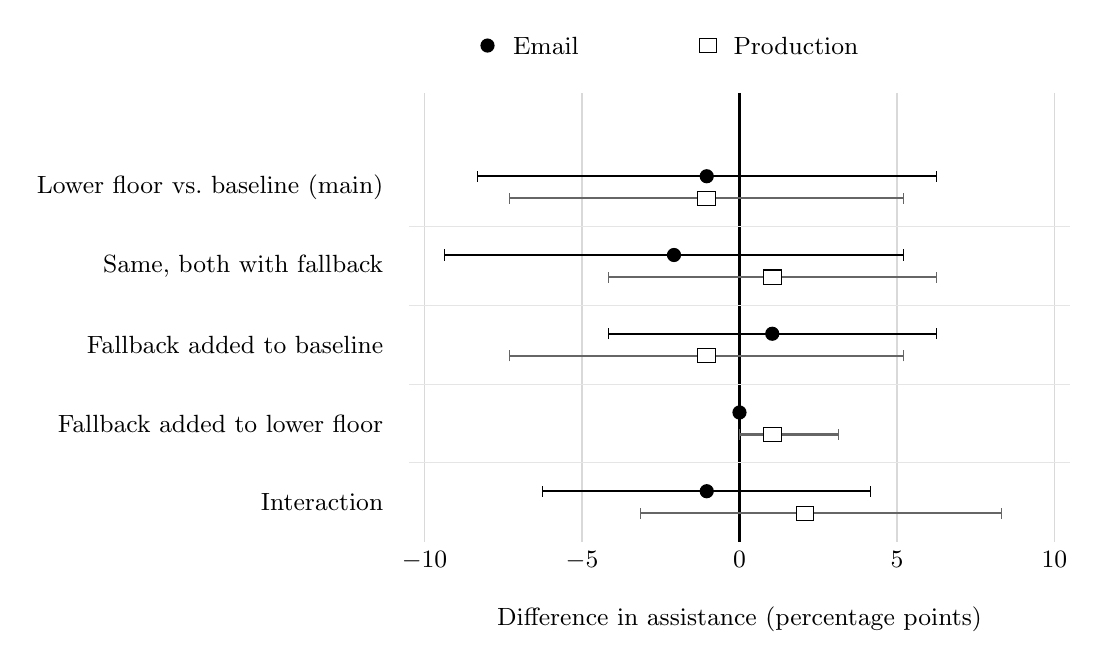
\begin{tikzpicture}[x=0.4cm,y=1cm,font=\small]
  \foreach \p in {-10,-5,0,5,10} {
    \draw[black!15] (\p,0.7) -- (\p,-5.0);
    \node[below] at (\p,-5.0) {$\p$};
  }
  \draw[thick] (0,0.7) -- (0,-5.0);
  \node[below] at (0,-5.7) {Difference in assistance (percentage points)};
  \node[left] at (-11,-0.5) {Lower floor vs.\ baseline (main)};
  \node[left] at (-11,-1.5) {Same, both with fallback};
  \node[left] at (-11,-2.5) {Fallback added to baseline};
  \node[left] at (-11,-3.5) {Fallback added to lower floor};
  \node[left] at (-11,-4.5) {Interaction};
  \foreach \y in {-1,-2,-3,-4} {
    \draw[black!10] (-10.5,\y) -- (10.5,\y);
  }
  % email: filled circle, upper offset
  \foreach \y/\m/\lo/\hi in {-0.36/-1.04/-8.33/6.25, -1.36/-2.08/-9.38/5.21, -2.36/1.04/-4.17/6.25, -3.36/0.00/0.00/0.00, -4.36/-1.04/-6.25/4.17} {
    \draw[thick] (\lo,\y) -- (\hi,\y);
    \draw (\lo,\y-0.07) -- (\lo,\y+0.07);
    \draw (\hi,\y-0.07) -- (\hi,\y+0.07);
    \fill (\m,\y) circle (0.9mm);
  }
  % production: open square, lower offset
  \foreach \y/\m/\lo/\hi in {-0.64/-1.04/-7.29/5.21, -1.64/1.04/-4.17/6.25, -2.64/-1.04/-7.29/5.21, -3.64/1.04/0.00/3.13, -4.64/2.08/-3.13/8.33} {
    \draw[thick,black!60] (\lo,\y) -- (\hi,\y);
    \draw[black!60] (\lo,\y-0.07) -- (\lo,\y+0.07);
    \draw[black!60] (\hi,\y-0.07) -- (\hi,\y+0.07);
    \draw[fill=white] (\m-0.28,\y-0.09) rectangle (\m+0.28,\y+0.09);
  }
  \fill (-8,1.3) circle (0.9mm);
  \node[right] at (-7.5,1.3) {Email};
  \draw[fill=white] (-1.28,1.21) rectangle (-0.72,1.39);
  \node[right] at (-0.5,1.3) {Production};
\end{tikzpicture}
\caption[Paired assistance differences between retrieval policies, with 95\% question-group bootstrap intervals, for the email and production samples]{Paired assistance differences between retrieval policies, with 95\% question-group bootstrap intervals, for the email and production samples. All intervals include zero. The email interval for adding the fallback to the lower floor is a single point at zero, because with the lower floor both fallback settings select identical contexts for all 96 questions. The values are in Table~\ref{tab:luna-effects}.}
\label{fig:policy-effects}
\end{figure}


Figure~\ref{fig:policy-effects} and Table~\ref{tab:luna-effects} show the differences between the policies, read as described in Section~\ref{sec:read-results}.

For the main comparison, the lower floor against the baseline, email has 5 questions that gain a good response, 6 that lose one and 85 that stay the same. Production has 4 gains, 5 losses and 87 unchanged. In both samples there is one more loss than gain, a difference of $-1.04$ points. The interval is $[-8.33, 6.25]$ for email and $[-7.29, 5.21]$ for production. Both include zero, so the data cannot tell whether the lower floor helps or hurts. They do rule out, under this judge, a gain larger than about 6 points for email and 5 for production. The sign test gives $p=1.0$ in both samples, the highest possible value, because 5 against 6 and 4 against 5 are as balanced as gains and losses can be. With the main judge's labels, the study therefore finds no clear benefit from the lower document threshold (for 2 further judges, see Section~\ref{sec:sonnet-rejudge}). It does not show that the policies are equal or that a better threshold cannot exist.

The other rows of the table repeat the comparison with the fallback on, and measure what adding the fallback does under each floor. The last row, the interaction, asks whether the fallback works differently under the two floors. It is the fallback's effect under the lower floor minus its effect under the baseline, $-1.04$ points for email and $+2.08$ for production. All of these intervals include zero.

The fallback is used much more often with the higher threshold of the baseline. Comparing the baseline with and without fallback, 33 email and 27 production cases change from an empty to a non-empty context. Comparing the lower floor with and without fallback, no email and only 3 production contexts change. With the lower floor, both fallback settings select the same context for all 96 email and 93 production cases. The zero email difference therefore comes from identical inputs and does not mean the fallback never matters. These counts are computed from the paired contexts.

\subsubsection{More evidence without a clear gain}
\label{sec:more-evidence}

The mean context grows from 5,110 to 16,481 characters for email and from 1,010 to 5,808 for production (Table~\ref{tab:context-diagnostics}), while the share of good answers stays the same. Even when no evidence is retrieved, the prompt still contains the list of useful links and the role instructions. This may explain why routing responses are still possible. Among the 55 empty contexts under the lower floor (3 email and 52 production), 23 still received a useful-routing label (3 email and 20 production).

\begin{table}[htbp]
\centering
\caption[Context measures for the main comparison]{Context measures for the main comparison. Context excludes the separate list of useful links.}
\label{tab:context-diagnostics}
\begin{tabular}{llrr}
\toprule
Sample & Measure & Baseline & Lower floor \\
\midrule
Email & Empty contexts & 36 & 3 \\
Email & Mean context characters & 5,110 & 16,481 \\
Email & Mean document candidates & 0.82 & 6.67 \\
Production & Empty contexts & 76 & 52 \\
Production & Mean context characters & 1,010 & 5,808 \\
\bottomrule
\end{tabular}
\end{table}

Empty contexts have 2 causes. Under the baseline, candidates were retrieved but none reached the 0.10 floor in 33 of the 36 empty email contexts and 27 of the 76 empty production contexts. Under the lower floor the document floor is 0.00, so these candidates are kept. For most contexts that stay empty under the lower floor, the saved replay holds no candidate at all (all 3 email and 49 of the 52 production contexts). Examples include greetings and very short or off-topic messages. In the other 3 production cases, only FAQ candidates were found and they fell below the FAQ floor of 0.10.

Among 66 email cases with valid, non-empty references, the mean share of the reference quotations that appear in the context rises from 0.486 under the baseline to 0.661 under the lower floor. All quotations are present in 18 cases under the baseline and 29 under the lower floor. Missing evidence is therefore not the only reason for weak answers. How the response combines conditions and handles uncertainty may also matter, but this was not tested. One case shows the pattern. To avoid picking a convenient example, it was chosen by a fixed rule that does not look at the outcomes. The rule chose among 72 cases that have a valid, non-empty reference, completed answers under both policies and a longer context under the lower floor. The question asks whether admission under a special category drops the tuition. The baseline selects 3 FAQ candidates and one document candidate (6,470 characters), and the lower floor selects 3 FAQ and 7 document candidates (17,979 characters). Both answers explain the exemption, separate it from other semester charges and advise contacting Student Services, and both keep the supported-answer label. Yet the reference says the question can only be partly answered, and its third required quotation is absent from both contexts. The case is an example and does not show how often extra evidence leaves outcomes unchanged.

The component study points the same way. There the separate-threshold policy ranked the relevant passages higher within the pool (Section~\ref{sec:component-study}), yet in this experiment no gain appears in the assessed answers. Better ranking therefore does not mean better assessed answers.

\subsubsection{Delivery, response time and cost}

The production telemetry comes from the deployed system, with the author's own test requests removed. It records 699 request events over 69 days, with a median generation time of 12.2 seconds, and 95 percent of requests finished within 37.2 seconds. The timing and cost figures describe the fixed path only, with median hosted-call times of 2.1 seconds for email and 1.5 for production. At planning rates of USD~2 per million input tokens and USD~12 per million output tokens, the 2 controlled campaigns used an estimated USD~31, excluding hosting and GPU costs. Chapter~\ref{ch:live} measures the deployed agent.

\subsection{Checks on the judging}
\label{sec:judge-checks}

The labels above come from one AI judge and from references written by the same model family. The checks in this section test how far they can be trusted. Their design comes first and their results follow.

\subsubsection{Design of the checks}

Five checks test the judging. Table~\ref{tab:check-design} lists what each one asks and which answers it uses. None of them uses human labels, so none can show which judge is right. Together they show where the labels are stable and where they depend on the judge or on the references.

\begin{table}[htbp]
\centering
\caption[Checks on the judging]{Checks on the judging. Luna is GPT-5.6 Luna, the main judge.}
\label{tab:check-design}
\small
\begin{tabularx}{\linewidth}{@{}>{\raggedright\arraybackslash}p{0.19\linewidth}>{\raggedright\arraybackslash}X>{\raggedright\arraybackslash}p{0.2\linewidth}>{\raggedright\arraybackslash}p{0.2\linewidth}@{}}
\toprule
Check & Question it answers & Judged by & Material \\
\midrule
Control answers & Does the judge give the expected label when the right label is known? & Luna, later also Qwen & 18 control answers and 12 Macedonian versions \\
Reference check & Do the references quote their sources correctly? & Code, no model & All 212 references \\
Repeated judgment & Does the judge give the same label a second time? & Luna & 48 answers \\
Local model & Does a different, small model agree with the judge? & Qwen & The same 48 answers \\
Further judges & Do the results hold under other judges? & Claude Sonnet 5.5 and GPT-6 Luna & All 393 answers \\
\bottomrule
\end{tabularx}
\end{table}

\textbf{Control answers.} These are 18 short answers that an AI coding agent (GPT-6 Astra) wrote from public FAQ text. Each was built to show one situation, such as a correct answer, a contradiction, a missing step or a claim that a request was submitted when nothing was done. Each comes with its own reference and with the category and flags a correct judge should give, so the judge's label can be compared with a known one. Twelve more controls ask 6 of the questions in Macedonian, once in Cyrillic and once in Latin script, to test whether the script changes the label. They were added to the plan before any answer was generated. The controls are development checks written by an AI, not a validated test set. Figure~\ref{fig:judgment-example} shows one of them.

\textbf{Repeated judgment and the local model.} Forty-eight answers were drawn at random with seed 24905309 (41 from the main study and 7 from the pilot). Luna judged each of them a second time with exactly the same messages, which shows how consistent one judge is with itself. The same messages also went to Qwen3-8B~\cite{yang2025qwen3} (Qwen from here on), a much smaller model run locally in a compressed 4-bit form. It ran with temperature zero, so it always picks its most likely next word, with a 1,024-token limit and no retry. This shows how much two different judges differ. Because the two disagreed substantially, Qwen was afterwards also run on the 30 controls. This extra check changes no main label and does not mean that the stricter model is correct.

\textbf{Further judges.} To test how much the results depend on the judge, every saved answer was judged again by 2 more models. Claude Sonnet 5.5 comes from a different family than the answers. GPT-6 Luna is the newer model of the same family, and it also answers questions in the live deployment. Both received exactly the same 2 messages as the main judge (Figure~\ref{fig:call-inputs}), with the same scoring rules afterwards, so only the model changed. GPT-6 Luna ran with the main judge's settings, a 1,024-token limit and no extra reasoning. Sonnet could use up to 4,096 tokens, without extended thinking. This check was added after the main results were known (Section~\ref{sec:method-deviations}).

\subsubsection{Control answers}

The primary judge reproduces the expected category for 17 of the 18 original controls and the expected flag for all 18. In the remaining case it labels useful routing as a supported answer. It also matches all 12 Macedonian versions. On the 30 control prompts Qwen matches the expected categories and flags on 14 of 18 original controls and 10 of 12 script versions. In all 6 mismatches, Qwen labels an omission, useful routing or an unnecessary refusal as unsupported. These are development checks on AI-written controls.

\subsubsection{Reference quality and the guard}
\label{sec:reference-quality}

Of 212 pilot and main references, 182 pass the quotation checks and 30 fail. In the main sample, 78 email and 88 production references pass (Table~\ref{tab:reference-states}). The guard changes a positive label to uncertain when the reference quotations fail their checks. It changes 47 otherwise positive policy records in the main sample, 32 for email and 15 for production. Policies reuse identical answers, so these records come from 28 unique answers. Under the baseline and the lower floor the email counts are 7 and 8, and production has 4 under each. The guard does not check whether a source is official or whether a passing reference is complete.

\begin{table}[htbp]
\centering
\caption[Main reference states]{Main reference states. Passing means the quotation checks pass. The institution has not approved the reference.}
\label{tab:reference-states}
\begin{tabular}{lrrrr}
\toprule
Sample & Not empty, passing & Empty, passing & Invalid & Total \\
\midrule
Email & 66 & 12 & 18 & 96 \\
Production & 25 & 63 & 8 & 96 \\
\bottomrule
\end{tabular}
\end{table}

The 182 passing references include 76 with no facts left, and 75 of the 166 passing references in the main sample are of this kind. Twenty of the 25 production supported-answer labels under both the baseline and the lower floor use empty references. A true completeness flag can therefore mean that there was no fact to miss.

A sensitivity analysis made afterwards accepts the supported-answer category only when its reference is valid and not empty, and keeps useful routing. Under this rule the totals of the baseline and the lower floor become 31 and 29 for email and 33 and 32 for production. The email difference is $-2.08$ points with interval $[-9.38,5.21]$. The production difference remains $-1.04$ with interval $[-7.29,5.21]$. The rule does not give a corrected accuracy, because it also removes appropriate responses that contain no facts. A check made afterwards found 32 of the 49 rejected main quotations in a different source block of the same pool and 17 nowhere in it. This can guide repairs to the references, and it changes no labels.

\subsubsection{Repeated and local judgments}
\label{sec:judge-consistency}

Table~\ref{tab:judge-agreement} shows the agreement. All 48 repeated Luna judgments returned outputs and 47 were valid. This leaves 47 category pairs, and one pair with an unspecified flag is left out of the material-claim agreement. Of 48 local Qwen judgments, 46 are valid, leaving 45 category pairs. Qwen flags an unsupported material claim in 23 pairs where Luna does not, and the reverse occurs once. Citation flags agree in 14 of 32 pairs with specified values.

\begin{table}[htbp]
\centering
\caption[Sensitivity of assessment under matched prompts and references]{Sensitivity of assessment with the same prompts and references. Neither comparison shows which judge is correct.}
\label{tab:judge-agreement}
\begin{tabular}{llrrr}
\toprule
Comparison & Measure & Agreement & Percent & $\kappa$ \\
\midrule
Luna repeat & Category & 35/47 & 74.5 & 0.648 \\
Luna repeat & Material flag & 40/46 & 87.0 & 0.340 \\
Local Qwen & Category & 13/45 & 28.9 & 0.134 \\
Local Qwen & Material flag & 20/44 & 45.5 & 0.104 \\
\bottomrule
\end{tabular}
\end{table}

The models differ in size, in quantization (a smaller numeric format for the model weights) and in how they read the rubric. The disagreement lowers confidence in the absolute scores. It does not mean that the stricter judge should replace the main one.

For the assistance labels, with the original guard and without pilot answers, repeated Luna agrees in 38 of 40 usable pairs (95.0\%), with 14 assistance labels in each run. Qwen agrees in 25 of 38 pairs (65.8\%). Nine losses and 4 gains reduce its assistance count from 13 to 8. The shared guard can inflate agreement. The check does not show which judge is correct and does not calculate the policy effect again.

\subsubsection{Two further judges}
\label{sec:sonnet-rejudge}

Sonnet gave a usable judgment for 363 of the 393 answers. The other 30 flagged an unsupported claim but chose another category, which the rules count as a failure, as they do for Luna's 7 such judgments. GPT-6 Luna gave a usable judgment for 359 answers. Its other 34 judgments broke the same rule, did not finish within the token limit or failed to parse, and count as failures too.

Table~\ref{tab:sonnet-rejudge} compares the assistance counts. Sonnet labels more answers as useful routing, so its totals are higher. GPT-6 Luna is the strictest of the three and labels more answers incomplete. Table~\ref{tab:judge-pairs} shows how often each pair of judges agrees. Here $\kappa$ (Cohen's kappa) is the agreement beyond what chance alone would give, where 0 means chance level and 1 means full agreement. No pair agrees on whether an answer counts as assistance for more than three quarters of the answers.

\begin{table}[htbp]
\centering
\caption[Assistance under the 3 judges]{Assistance under the 3 judges, out of 96 questions per sample. Luna is GPT-5.6 Luna, the main judge. The last column is the difference between the lower floor and the baseline in percentage points, with the 95\% interval in brackets.}
\label{tab:sonnet-rejudge}
\small
\begin{tabular}{@{}llrrrrr@{}}
\toprule
Sample & Judge & Baseline & + fallback & Lower floor & + fallback & Difference \\
\midrule
Email & Luna & 31 & 32 & 30 & 30 & $-1.04$ $[-8.3, 6.3]$ \\
Email & Sonnet & 40 & 34 & 41 & 41 & $+1.04$ $[-7.3, 9.4]$ \\
Email & GPT-6 Luna & 21 & 21 & 19 & 19 & $-2.08$ $[-9.4, 5.2]$ \\
\addlinespace
Production & Luna & 53 & 52 & 52 & 53 & $-1.04$ $[-7.3, 5.2]$ \\
Production & Sonnet & 54 & 58 & 61 & 62 & $+7.29$ $[1.0, 13.5]$ \\
Production & GPT-6 Luna & 37 & 37 & 36 & 36 & $-1.04$ $[-5.2, 3.1]$ \\
\bottomrule
\end{tabular}
\end{table}

\begin{table}[htbp]
\centering
\caption[Agreement between the judges]{Agreement between each pair of judges on the answers for which both gave a usable judgment. Assistance agreement compares only whether the answer counts as assistance, and category agreement compares the exact outcome category.}
\label{tab:judge-pairs}
\small
\begin{tabular}{@{}lrrr@{}}
\toprule
Judges & Answers & Assistance agreement & Category agreement \\
\midrule
Luna and Sonnet & 358 & 72.3\% ($\kappa=0.45$) & 55.0\% ($\kappa=0.40$) \\
Luna and GPT-6 Luna & 354 & 74.0\% ($\kappa=0.48$) & 57.9\% ($\kappa=0.45$) \\
Sonnet and GPT-6 Luna & 334 & 66.8\% ($\kappa=0.38$) & 53.0\% ($\kappa=0.40$) \\
\bottomrule
\end{tabular}
\end{table}

The main comparison depends on the judge. For email, no judge finds a clear effect of the lower document threshold. For production questions, Sonnet finds a gain of 7.29 points, with an interval that excludes zero, while both Luna models find none. Sonnet also finds that the fallback lowers email assistance under the baseline ($-6.25$ points, interval $[-12.5,-1.0]$). Ten comparisons were made per judge, so an interval that excludes zero can appear by chance. Still, the conclusion that the lower document threshold gives no benefit holds under 2 of the 3 judges and not under Sonnet. GPT-6 Luna judges far fewer answers as useful than the other two, yet its policy differences match those of the main judge. The judges therefore disagree more on how good the answers are than on which policy is better, with Sonnet's production result as the exception.

\subsection{The prompt comparison}

\subsubsection{Design}
\label{sec:method-prompt}

A second, smaller experiment, the prompt comparison, compares a baseline prompt with a revised one. Where both are meant, the thesis calls them the controlled experiments. Neither is the deployed prompt. It runs on snapshot B, a read-only snapshot of 74 FAQs, 60 documents and 2,391 chunks, with 40 further emails that were not in the main sample, and with strict completion as its main measure. The FAQ text matches the controlled experiment, but the document set is larger. The comparison asks whether the revised prompt improves strict completion on the 40 emails.

A 32-question development sample, balanced between email and production questions, compared current retrieval, AI-selected reference evidence and no evidence. Giving the model AI-selected evidence instead of normal retrieval raised the reference facts covered by the answers from 29/73 to 50/73, and strict completion rose from 4/32 to 6/32. With no evidence at all, the answers reached 4/32 strict completions and 14/73 facts. This development work led to a revision of the prompt only, fixed before the comparison. The revised prompt checks dates and whether a rule applies to the student, instead of automatically favoring FAQs or higher-ranked text. It also keeps needed steps of a procedure and states important gaps.

The 40 emails are the first 40 of a shuffled reserve of 64 archive emails kept apart from the main sample, after exact and near duplicates of evaluated questions were removed. It is not proved that they differ in meaning from the evaluated ones. Two passes of Luna prepared and reviewed the references before generation, and all 40 references pass exact-text checks (34 partial, 3 insufficient, 3 not factual). Both conditions use production retrieval with the fallback enabled, useful links, Luna, the gateway's default sampling and a 1,536-token limit. Strict completion is stricter than the assistance measure and cannot be compared with it. Paired differences use 20,000 bootstrap samples (Section~\ref{sec:read-results}) and an exact paired test on the cases where the 2 conditions differ.

\subsubsection{Results}
\label{sec:results-prompt}

In the 40-question comparison the first judge did not see part of the evidence given to the generator. It flagged 15 citation errors per condition, while a rule-based check found one per condition. All pairs were therefore graded again with the full generation context, new scope guidance and a 1,024-token limit on the judgment (Section~\ref{sec:method-deviations}). This audit is the reported result (Table~\ref{tab:prompt}).

\begin{table}[t]
\centering\small
\caption[Forty-question prompt comparison]{Forty-question prompt comparison. Audit means the repeated assessment with the full generation evidence.}\label{tab:prompt}
\begin{tabular}{lrr}
\toprule
Measure & Current prompt & Revised prompt\\
\midrule
Completed generations & 37/40 & 37/40\\
Initial strict completions (incomplete judge evidence) & 4/40 & 6/40\\
Audit strict completions & 6/40 & 5/40\\
Audit unsupported-claim flags & 15/37 & 10/36\\
Audit citation-error flags & 1/37 & 1/36\\
\bottomrule
\end{tabular}
\end{table}

Under the audit the revised prompt changes strict completion from 6/40 to 5/40. The paired difference is $-2.5$ points (95\% bootstrap interval $[-12.5,7.5]$), from 2 gains and 3 losses, and an exact sign test gives $p=1.0$. The 5-point gain under the first labels may have come from the judge's incomplete input, so it is not a finding about the prompt. The audit also changed the scope guidance and the token limit, so the change in labels cannot be put down to the evidence alone. Three inputs that were too long produce no answer in either condition but still count in the totals. Because the references are partial, fewer unsupported-claim flags do not show an improvement.

\subsection{Changes to the plan}
\label{sec:method-deviations}

The plan of the controlled experiment was fixed before any evaluated answer was generated. It fixed the sample and seed, the 4 policies, the main comparison of the lower floor against the baseline, how references and judgments are made, the outcome categories and the analysis. A fingerprint (hash) of every input file was saved, so later changes would show. An addition, also written down before generation, added the 12 Macedonian script controls and the input-rejection outcome for the 4 questions that were too long. It changed no threshold or rubric. The prompt comparison had its own plan, and its revised prompt was fixed before it ran.

The executed assessment differs from the first design in 3 ways. It uses a compact judgment format instead of one entry per claim, repeats 48 assessments instead of 24, and leaves out a proposed fifth policy with a tuned threshold. Six steps were added after the results were seen. They are marked as such and replace no main result. The research questions were reworded, with the same hypotheses, policies, outcomes and labels. Three extra checks were run: the analysis without empty references, the Qwen run on the 30 control prompts, and the search for rejected reference quotations. The prompt comparison was graded a second time. Finally, all answers were judged again by Claude Sonnet 5.5 and by GPT-6 Luna, with the same messages as the main judge (Section~\ref{sec:sonnet-rejudge}).

The saved records allow every reported count and interval to be calculated again without new model calls. The chatbot-log questions and the generated answers are not released, and calling the hosted model again would not necessarily give the same text. The controlled experiment lacks a complete database snapshot, while the prompt comparison keeps one.

\paragraph{Summary.}
\begin{itemize}
  \item Four policies cross a document score floor with a fallback rule on the fixed pipeline, which does not evaluate the deployed system. One shared AI reference and one anonymous AI judge produce the labels, and no check is human validation.
  \item Under the baseline and the lower floor, incomplete answers (22 to 31 of 96 per sample) and unsupported claims (11 to 20) remain common.
  \item Lowering the document threshold raises the mean context from 5,110 to 16,481 characters for email and from 1,010 to 5,808 for production, but the share of good answers does not rise. The main effect is $-1.04$ points in both samples, and every interval includes zero.
  \item The same change ranks relevant passages higher in the component study, so better ranking does not mean better assessed answers.
  \item Many passing references are empty, and the judge's inputs and strictness can move the apparent results.
  \item Judged again by Claude Sonnet 5.5, the lower document threshold shows a 7.29-point gain for production questions, while GPT-6 Luna, like the main judge, finds none. The main result therefore depends on the judge.
\end{itemize}
